% !TeX program = lualatex
% !TeX root = luaking.tex
% !TeX encoding = UTF-8
% !TeX spellcheck = cs_CZ
%---------------------------------------------------------------------------------------------------
% file fey1ch18.tex
%---------------------------------------------------------------------------------------------------
%=========================== Kapitola: Dvojrozměrná rotace =========================================
\setchaptertoc
\chapter{Dvojrozměrná rotace}\label{fyz:IchapXVIII}
  \section{Hmotný střed}\label{fyz:IchapXVIIIsecI}
    V předcházejících kapitolách jsme studovali mechaniku hmotných bodů, malých částic, Jejichž
    vnitřní struktura nás nezajímá. V několika dalších kapitolách budeme aplikovat Newtonovy Zákony
    na komplikovanější objekty. Když se příroda, díky novým poznatkům stává pro člověka
    komplikovanější, Stává se i zajímavější a uvidíme, že jevy, týkající se mechaniky komplexnějších
    objektů, než jsou hmotné body, jsou docela překvapující. Samozřejmě, v těchto jevech se
    neprojevuje nic jiného než kombinace Newtonových zákonů, ale někdy je těžké uvěřit, že přitom
    uplatňuje jen \(F= ma\).
    
    Komplikovanější objekty, jimiž se budeme zabývat, mohou být různé: proudění vody, otáčení
    galaxií apod. Začneme s analýzou nejjednoduššího „komplikovaného“ objektu, jenž nazýváme tuhým
    tělesem - je to pevný předmět, jenž se při svém pohybu otáčí. Avšak i pohyb takovéhoto
    jednoduchého objektu může být velmi složitý. Proto se nejdříve budeme Zabývat nejjednoduššími
    stránkami takového pohybu - když těleso rotuje kolem pevně osy. V takovém tělese se pak daný bod
    pohybuje v rovině kolmé k této ose. Taková rotace tělesa kolem pevné osy se nazývá rovinnou nebo
    dvojrozměrnou rotaci. Získané výsledky zobecníme i na trojrozměrné rotace, ale přitom zjistíme,
    že na rozdíl od obyčejné mechaniky částice, jsou rotace „rafinovanější“ a těžko pochopitelné,
    nepochopíme-li je dostatečně v dvojrozměrném případě.

    K prvnímu zajímavému poznatku můžeme dojít, když do vzduchu hodíme objekt, skládající se z
    množství kvádrů a tyčí, jež jsou navzájem spojeny vlákny. Samozřejmě víme, že se bude pohybovat
    po parabole, neboť jsme to zjistili při studiu pohybu jedné částice. Nyní naše těleso není
    jednou částicí a ačkoli rotuje, poskakuje apod., lze vidět, že se pohybuje po parabole. Co se
    vlastně pohybuje po parabole? Určitě ne bod v rohu kvádru, neboť ten poskakuje sem a tam, ani
    bod na konci dřevěné tyče nebo v jejím středu či ve středu kvádru. Něco se však po parabole
    pohybuje, jakýsi zdánlivý střed. Naše první věta, týkající se komplikovaných objektů říká, že
    existuje nějaký „střed“, který lze matematicky definovat. Pohybuje se po parabole a nemusí to být
    bod v samotném tělese. Je to věta o hmotném středu a její důkaz nyní následuje.

    Každé těleso se skládá z množství malých částic - atomů, mezi nimiž působí různé síly. Označme
    si jednu z částic indexem \(i\). (jsou jich miliony, takže \(I\) nabývá např. hodnoty do
    \num{e23}). Síla, jež působí na \(i\)-tou částici, je pak rovna hmotnosti částice vynásobené
    jejím zrychlením
    \begin{equation}\label{fyz:eq649}
      \vr{F}_i=m_i\dder{\vr{r}_i}{t}.
    \end{equation}
   
    V několika následujících kapitolách budeme hovořit o pohybu, při němž rychlosti pohybu těles a
    jejich částic jsou mnohem menší, než je rychlost světla, a všechny veličiny budeme používat v
    nerelativistickém přiblížení. Za těchto okolností je hmotnost konstantní, takže
    \begin{equation}\label{fyz:eq650}
      \vr{F}_i=\dder{(m_i\vr{r}_i)}{t}.
    \end{equation}
    Sečteme-li síly působící na všechny částice, tj. když najdeme součet všech \(\vr{F}_i\) pro
    všechny možné indexy, dostaneme výslednou sílu \(\vr{F}\). Na druhé straně rovnice dostaneme
    totéž, jako kdybychom nejprve sčítali a pak diferencovali:
    \begin{equation}\label{fyz:eq651}
      \sum_i\vr{F}_i=\vr{F}=\dder{\left(\sum_im_i\vr{r}_i\right)}{t}.
    \end{equation}
    Výsledná síla je proto rovna druhé derivaci součtu součìnů hmotností a jejich poloh.

    Výsledná síla, působící na všechny částice je vlastně stejná, jako vnější síla. Proč? Ačkoli na
    částice působí různé síly (tah vláken, nárazy, atomové síly a kdoví co ještě) a to všechno
    musíme sečíst dohromady. Naštěstí nás Zachraňuje třetí Newtonův zákon. Akce a reakce mezi
    libovolnými dvěma částicemi je stejná, takže sečteme-li všechny rovnice, vyruší se v součtu síly
    mezi kterýmikoli dvěma částicemi a konečný výsledek představuje ty Síly, jež jsou způsobeny
    jinými částicemi, ne těmi, jež tvoří těleso. Takže jestliže rovnice (\ref {fyz:eq651}) je
    součtem přes určitý počet částic, jež spolu tvoří „dané těleso“, pak \emph{vnější} síla, která
    působí na celé těleso, je rovna součtu všech sil působících na všechny částice tělesa.

    Bylo by nyní hezké, kdybychom mohli rovnici (\ref {fyz:eq651}) napsat jako součin celkové
    hmotnosti a nějakého zrychlení, což také můžeme provést. Řekněme, že \(M\) je celková hmotnost,
    tj. součet hmotností všech částic. Definujeme-li vektor \(R\) tak, aby
    \begin{equation}\label{fyz:eq652}
      \vr{R}=\frac{\sum_im_i\vr{r}_i}{M}.
    \end{equation}
    pak rovnice (\ref {fyz:eq651}) bude prostě
    \begin{equation}\label{fyz:eq653}
      \vr{F}=\dder{(M\vr{R})}{t}=M\dder{\vr{R}}{t},
    \end{equation}
    protože \(M\) je konstanta. Zjistili jsme, že vnější síla je rovna celkové hmomosti násobené
    zrychlením nějakého pomyslného bodu, jehož poloha je R. Tento bod se nazývá \textbf{hmotný střed
    tělesa}\footnote{Ve fyzice se často místo termínu „hmotný střed“ nebo také \uv{střed hmotnosti}
    používá kratšího termínu „těžiště“. I když přesně vzato, oba termíny neoznačují totéž (těžiště
    lze určovat jen v homogenním tíhovém poli, zpravidla taková záměna názvů nepůsobí potíže. }. Je
    to bod někde „uprostřed“ tělesa, určité průměrné \(\vr{r}\), přičemž důležitost jednotlivých
    vektorů \(\vr{r}_i\) je úměrná jejich hmotnostem. 

    Význam této věty probereme podrobněji v některé další kapitole. Nyní se omezíme na dvě poznámky:
    Za prvé, jsou-li vnější síly nulové a vznáší-li se těleso v prázdném prostoru, může se otáčet,
    vrtět a dělat různé pohyby, ale \emph{hmotný střed}, tato uměle vytvořená vypočítaná poloha
    někde uprostřed tělesa, \emph{se bude pohybovat konstantní rychlostí}. Ve zvláštním případě,
    byl-li původně v klidu, zůstane v klidu. Máme-li tedy nějakou krabici nebo kosmickou loď s
    lidmi, vypočítáme její hmotný střed a zjistíme, že je v klidu, pak jestliže na kosmickou loď
    nepůsobí vnější síly, hmotný střed bude nadále setrvávat v klidu. Samozřejmě, kosmická loď se
    přitom může mírně pohybovat v prostoru, ale jen proto, že lidé uvnitř chodí sem a tam. Když
    někdo půjde dopředu, loď se posune dozadu tak, aby střední poloha všech hmot zůstávala na témž
    místě. Je proto pohon rakety absolutně nemožný, když nemůžeme zevnitř pohnout hmotným středem?
    Ne, ale vyplývá z toho, že když chceme pohnout tou částí rakety, kterou potřebujeme, musíme její
    nepotřebnou část odstranit. jinými slovy, má-li raketa na začátku nulovou rychlost a
    vymrštíme-li ven nějaký plyn, tento malý obláček plynu se bude pohybovat jedním směrem a raketa
    opačným, ale hmotný střed zůstane přesně tam, kde byl předtím. Takže potřebná část rakety se
    pohybuje opačně než nepotřebná.

    Druhá poznámka týkající se hmotného středu a důvod, proč jsme v naší souvislosti tento pojem
    zavedli, je ta, že pohyb hmotného středu je možno uvažovat odděleně od „vnitřních“pohybů tělesa,
    a proto se jím v naší diskuzi o rotacích nemusíme zabývat.
  
  \section{Rotace tuhého tělese}\label{fyz:IchapXVIIIsecII}
    Nyní pojďme studovat rotace. Obyčejné těleso samozřejmě nevykonává jen jednoduchý rotační pohyb,
    ale ohýbá se, chvěje se a deformuje. Proto, abychom si věci zjednodušili, budeme hovořit o
    pohybu neexistujícího ideálního tělesa, které nazýváme tuhým tělesem. Je to takové těleso, v
    němž jsou síly mezi atomy tak silné a mají takový charakter, že slabé síly, potřebné k jeho
    uvedení do pohybu, ho nezdeformují. Při pohybu si tuhé těleso zachovává v podstatě stejný tvar.
    Chceme-li studovat pohyb takového tělesa a přitom ignorovat pohyb hmotného středu, zůstává jen
    jedna věc, kterou ještě můžeme studovat - a to je \textbf{rotace}. Jak ji máme popsat.
    Předpokládejme, že v tělese je dána nějaká přímka, která může procházet hmotným středem, ale
    nemusí, a těleso rotuje kolem této přímky jako kolem osy. jak definujeme rotaci? To je dost
    jednoduché, neboť když si kdekoli v tělese označíme bod (mimo osu) a když víme, kam se tento bod
    posunul, můžeme vždy přesně říci, kde se těleso nachází. Jediné, co potřebujeme znát, abychom
    popsali polohu tohoto bodu, je nějaký \emph{úhel}. Studium rotace je proto studiem změn tohoto
    úhlu s časem.

    Když studujeme rotaci, pozorujeme, o jaký úhel se těleso otočilo. Nejde nám přitom o jakýkoli
    úhel \emph{uvnitř} tělesa, nejde o to, abychom měřili nějaký úhel na tělese. Jde nám o
    \emph{úhlovou změnu polohy} celého tělesa za nějakou dobu.

    Nejdříve budeme studovat kinematiku rotací. Úhel se bude měnit v závislosti na čase a právě tak,
    jak jsme hovořili o poloze a rychlosti v jednorozměrném případě, můžeme hovořit o úhlové poloze
    a úhlové rychlosti v případě rovinné rotace. Mezi dvojrozměrnými rotacemi a jednorozměrným
    pohybem skutečně existuje velmi zajímavý vztah, v němž téměř každá veličina má svou analogii.
    Známe úhel \(\varTheta\), který určuje, jak se těleso \emph{otočilo}; ten nahrazuje vzdálenost
    \(y\), která určuje, jak daleko se těleso posunulo. Podobně známe rychlost otáčení \(\omega=
    \der{\varTheta}{t}\), která říká, jak se změní úhel za sekundu, podobně jako \(v = \der{s}{t}\)
    popisuje rychlost pohybu tělesa nebo velikost posunutí za sekundu. Jestliže se úhel měří v
    radiánech, bude úhlová rychlost \(\omega\) tolik a tolik radiánů za sekundu. Čím je úhlová
    rychlost větší, tím rychleji se těleso otáčí a tím rychleji se mění úhel. Můžeme pokračovat:
    úhlovou rychlost můžeme derivovat podle času a \(\varepsilon = \der{\omega}{t} =
    \dder{\varTheta}{t}\) můžeme nazvat úhlovým zrychlením. To by byla analogie obyčejného
    zrychlení.

    \begin{figure}[ht!] %\ref{fyz:fig398}
      \centering
      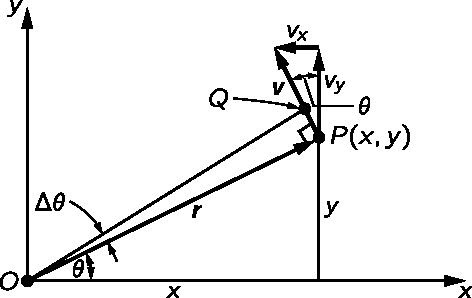
\includegraphics[width=0.9\linewidth]{fyz_fig398.pdf}
      \caption{Kinematika dvojrozměrné rotace (\cite[s.~251]{Feynman01})}
      \label{fyz:fig398}
    \end{figure}
    
    Nyní budeme muset dát do souvislosti dynamiku rotace s dynamickými zákony částic tvořících
    těleso. K tomu potřebujeme zjistit, jak se pohybuje určitá částice, když má danou úhlovou
    rychlost. Proto si vybereme částici, jež se nachází ve vzdálenosti \(r\) od osy, a řekněme, že v
    daném okamžiku má určitou polohu \(P( x, y)\) (obr. \ref{fyz:fig398}). Pootočil-li se za dobu
    \(\Delta t\)  úhel celého tělesa o \(\Delta\varTheta\), posunula se s ním i částice. Nachází se
    ve stejné vzdálenosti od \(\varTheta\) jako předtím, jen se dostala do bodu \(Q\). První, co nás
    zajímá je, oč se změní vzdálenost \(x\) a vzdálenost \(y\). Označíme-li \(OP\) jako \(r\), pak
    vzdálenost \(PQ\) je \(r\Delta\varTheta\), neboť tak je definován úhel. Změna \(x\) je prostě
    projekcí \(r\Delta\varTheta\) do směru osy \(x\):
    \begin{equation}\label{fyz:eq654}
      Δx=−PQ\sin\varTheta =−rΔ\varTheta\cdot\frac{y}{r}=−yΔ\varTheta.
    \end{equation}
    Podobně
    \begin{equation}\label{fyz:eq655}
      Δy=−x\Delta\varTheta.
    \end{equation}
    Otáčí-li se těleso s danou úhlovou rychlostí \(\omega\), pak dělením obou stran rovnic
    (\ref{fyz:eq654}) a (\ref{fyz:eq655}) \(\Delta t\) najdeme, že rychlost částice je
    \begin{equation}\label{fyz:eq656}
      v_x=−ωy \qquad\text{a}\qquad v_y=+ωx.
    \end{equation}
    Chceme-li zjistit velikost rychlosti, musíme napsat
    \begin{align}
      v&=\sqrt{v^2_x+v^2_y}=\sqrt{ω^2y^2+ω^2x^2} \nonumber\\
       &=ω\sqrt{x^2+y^2}=ωr.                     \label{fyz:eq657}
    \end{align}
    Nemělo by se zdát divné, že velikost .této rychlosti je \(\omega r\). Vlastně by to mělo být
    samozřejmé, neboť vzdálenost, o jakou se bod posunul, je  \(rΔ\varTheta\) a vzdálenost, o niž se
    posune za sekundu, je \(rΔ\varTheta/Δt\) neboli \(r\omega\).

    Pojďme dále a podívejme se na dynamiku rotace. Musíme zavést novou veličinu - sílu. Ptáme se,
    zda můžeme vynalézt něco, co budeme nazývat torzní silou (z latinského slova torquere; česky
    točit, kroutit) nebo \textbf{momentem síly}, což by mělo stejný vztah k rotaci, jako má síla k
    posuvnému pohybu. Tak jako síla vyvolává posuvný pohyb, moment síly je něco, co vyvolává rotaci.
    Kvalitativně představuje moment síly rotaci, ale jak ho vyjádřit kvantitativně? Kvantitativní
    vyjádření momentu síly dostaneme, když budeme zkoumat \emph{práci} vykonanou při otočení tělesa.
    Vždyť jeden velmi pěkný způsob, jak definovat sílu, je vyjádřit práci, kterou vykoná, když
    způsobí nějaké posunutí. Analogií mezi veličinami posuvného a rotačního pohybu se pokusíme
    zachovat tak, že práci, vykonanou při rotaci, položíme rovnu součinu \emph{momentu síly a úhlu},
    o který se těleso pootočilo. Jinak řečeno, definice momentu síly bude taková, že věta o práci
    bude mít svou analogii: síla krát vzdálenost je práce, a i moment síly krát úhel bude rovněž
    práce. To nám říká, co je to moment síly. Na chvíli si představme nějaké tuhé těleso, na něž
    působí různé síly, a nějakou osu kolem níž se těleso otáčí. Nejdříve se soustřeďme na jednu sílu
    a předpokládejme, že působí v bodě \((x, y)\). Jaká práce by se vykonala, kdybychom těleso
    pootočili o velmi malý úhel? Zcela snadno určíme, že vykonaná práce je
    \begin{equation}\label{fyz:eq658}
      ΔW=F_xΔx+F_yΔy.
    \end{equation}
    Stačí dosadit za \(Δx\) a \(Δy\) z rovnice (\ref{fyz:eq654}) a (\ref{fyz:eq655}) a dostaneme
    \begin{equation}\label{fyz:eq659}
      ΔW=(xF_y−yF_x)Δ\varTheta.
    \end{equation}
    Vykonaná práce je proto ve skutečnosti rovna úhlu, o který jsme těleso pootočili, vynásobenému
    podivnou kombinací složek síly a vzdálenosti, již nazýváme momentem síly. Definice práce při
    malém pootočení jako součinu momentu síly a úhlu, určuje i vzorec pro vyjádření momentu síly
    pomocí síly. (Je jasné, že moment síly nepředstavuje zcela novou myšlenku, nezávislou na
    Newtonově mechanice - proto se musí moment síly definovat pomocí síly.)

    Působí-li na těleso více sil, pak vykonaná práce \(\Delta W\) je samozřejmě rovna součtu prací
    vykonaných všemi silami, z nichž \emph{každá práce je úměrná} \(\Delta \varTheta\). Proto můžeme
    \(\Delta \varTheta\) vytknout ze součtu a lze říci, že malá práce je rovna součtu všech momentů
    sil (jež existují díky všem různým silám působícím na těleso) vynásobenému \(\Delta \varTheta\).
    Tento součet můžeme nazvat celkovým momentem síly \(N\). Takže momenty sil se sčítají podle
    běžných pravidel algebry, ale později uvidíme, že jen proto, že pracujeme v rovině. Je to jako v
    jednorozměrné kinematice, kde se všechny síly sčítají algebraicky, ale jen proto, že mají
    všechny stejný směr. Ve třech rozměrech je to komplikovanější. Takže v dvojrozměrné rotaci platí
    \begin{equation}\label{fyz:eq660}
      τ_i=x_iF_{y_i}−y_iF_{x_i}
    \end{equation}
    a 
    \begin{equation}\label{fyz:eq661}
      τ=∑τ_i.
    \end{equation}
    Musíme zdůraznit, že jde o moment síly vzhledem k dane ose. Kdybychom zvolili jinou osu, takže
    všechna \(x_i\) a \(y-i\) by se změnily, pak by se změnila (obyčejně) i velikost momentu síly.

    Nyní si krátce všimneme, že takto pomocí práce zavedený moment síly nám poskytuje velmi
    důležitý výsledek pro tělesa v rovnováze: jsou-li všechny síly, jež působí na těleso, v
    rovnováze, z hlediska translace i rotace, pak je nulová nejen výsledná síla, ale i součet všech
    \emph{momentů sil} Nachází-li se totiž těleso v rovnovážném stavu, pak při malém posunutí
    nevykonávají síly žádnou práci. Proto když platí \(ΔW=τΔθ=0\), musí být součet všech momentů sil
    nulový. Na rovnovážný stav se vztahují dvě podmínky: výslednice sil je rovna nule a výslednice
    momentů sil je rovna nule. 

    \begin{figure}[ht!] %\ref{fyz:fig399}
      \centering
      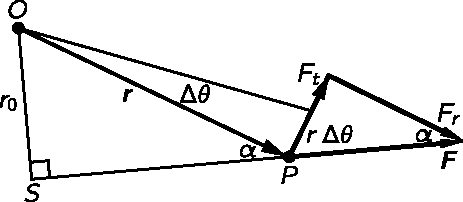
\includegraphics[width=0.9\linewidth]{fyz_fig399.pdf}
      \caption{K momentu síly (\cite[s.~253]{Feynman01})}
      \label{fyz:fig399}
    \end{figure}

    Nyní si představme jedinou sílu a pokusme se znázornit si geometricky, co to je ten zvláštní
    výraz \( xF_y−yF_x\). Síla \(\vr{F}\) působící v bodě \(\vr{r}\) je znázorněn na obr.
    \ref{fyz:fig399}. Práce vykonaná při pootočení tělesa o malý úhel \( Δθ\) je rovna součinu
    složky síly ve směru posunutí a tohoto posunutí. Jinými slovy, uplatňuje se pouze tangenciální
    složka síly a tu je třeba násobit vzdáleností \( rΔθ\). Proto je i moment síly roven
    tangenciální složce síly (kolmé na poloměr) násobené poloměrem. To souhlasí s naší původní
    koncepcí momentu síly, neboť kdyby síla byla zcela radiální, nemohla by těleso vůbec otočit. je
    jasné, že kroutící efekt by měl být způsoben jen tou částí síly, jež nepůsobí směrem od osy, to
    znamená její tangenciální složkou. Dále je jasné, že daná síla je účinnější na dlouhém rameni
    než blízko u osy. Skutečně, kdybychom působili přímo na osu, těleso vůbec neotočíme! Takže je
    zcela rozumné, když řekneme, že velikost momentu síly je úměrná radiální vzdálenosti a
    tangenciální složce síly.

    Existuje ještě třetí velmi zajímavý vztah pro moment síly. Právě jsme viděli, že moment síly
    je síla krát poloměr krát sinus úhlu \(\alpha\) (obr. \ref{fyz:fig399}). Když ale prodloužíme
    přímku, po níž působí síla, a kolmo k této přímce nakreslíme úsečku OS (\textbf{rameno síly}),
    uvidíme, že toto rameno síly je kratší než \(r\) právě v takovém poměru, v jakém je tangenciální
    složka síly menší než celá síla. Proto můžeme moment síly vyjádřit i jako velikost síly
    násobenou ramenem síly.

    Původ názvu momentu síly je nejasný, ale je možná odvozen z latinského \emph{movimentum}, pohyb
    a schopnost síly pohnout tělesem (působením na páku nebo sochor) je tím větší, čím je delší
    rameno síly. V matematice „moment“ znamená váhový faktor vyjadřující vzdálenost od osy.    

  \section{Moment hybnosti}\label{fyz:IchapXVIIIsecIII}
    Ačkoli jsme zatím brali v úvahu jen speciální případ tuhého tělesa, jsou vlastností momentů sil
    a jejich matematických vztahů zajímavé dokonce i tehdy, kdy tělesa nejsou tuhá. Skutečně, lze
    dokázat velmi zajímavou větu: Právě tak, jako vnější síla je dána rychlostí změny veličiny
    \(p\), již nazýváme celkovou hybností skupiny částic, tak i vnější moment síly je dán rychlostí
    změny veličiny \(L\), již nazýváme \textbf{momentem hybnosti} skupiny částic.
  
    \begin{figure}[ht!] %\ref{fyz:fig400}
      \centering
      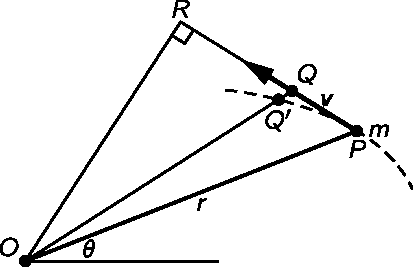
\includegraphics[width=0.9\linewidth]{fyz_fig400.pdf}
      \caption{Částice pohybující se kolem osy \(O\) (\cite[s.~254]{Feynman01})}
      \label{fyz:fig400}
    \end{figure}

    Abychom to dokázali, budeme předpokládat, že máme částice, na něž působí nějaké síly, a
    zjistíme, co se s nimi bude dít pod vlivem momentů těchto sil. Samozřejmě, nejdříve bychom měli
    uvažovat jen jednu částici. Na obr. \ref{fyz:fig400} je znázorněna částice o hmotnosti \(m\) a
    osa \(O\). Není nutné, aby se částice pohybovala kolem \(O\) po kružnici, může se pohybovat po
    elipse jako planeta kolem Slunce nebo po jiné dráze. Částice se nějak pohybuje, působí na ni
    síly, které ji zrychlují podle obvyklého vztahu: složka síly ve směru osy \(x\) je rovna
    hmotnost krát složka zrychlení ve směru \(x\) atd. Ale podívejme se, co způsobí moment síly.
    Moment síly je roven \( xF_y−yF_x\) a síla ve směru osy \(x\) nebo \(y\) je hmotnost krát
    zrychlení ve směru osy \(x\) nebo \(y\)
    \begin{equation}\label{fyz:eq662}
      τ = xF_y−yF_x = xm\cdot\dder{y}{t}−ym\cdot\dder{x}{t}. 
    \end{equation}
    I když se nezdá, že by to byla derivace nějaké jednoduché veličiny, je to derivace rozdílu
    \(xm\left(\der{y}{t}\right) - ym\left(\der{x}{t}\right)\). Ukažme to:
    \begin{equation}
      \begin{split}
        \der{}{t}
          &\left[xm\left(\der{y}{t}\right)- ym\left(\der{x}{t}\right)\right]               \\                                       \\
          &= xm\left(\dder{y}{t}\right) + \left(\der{x}{t}\right)m\left(\der{y}{t}\right)  \\
          &- ym\left(\dder{x}{t}\right) - \left(\der{y}{t}\right)m\left(\der{x}{t}\right)  \\
          &= xm\left(\dder{y}{t}\right) - ym\left(\dder{x}{t}\right).      \label{fyz:eq663} 
      \end{split}
    \end{equation}

    Je tedy pravda, že moment síly je roven rychlosti změny něčeho v závislosti na čase. Všimněme
    si toho „něčeho“ a dejme tomu jméno: \textbf{moment hybnosti} \(L\):
    \begin{equation}\label{fyz:eq664}
      L=xm\der{y}{t} − ym\der{x}{t} = xp_y−yp_x.
    \end{equation}

    Ačkoli tato naše úvaha není relativistická, druhý výraz v této rovnici platí i v teorii
    relativity. Zjistili jsme tedy, že existuje rotační analogie i pro hybnost a tato analogie -
    moment hybnosti - je určena prostřednictvím složek hybnosti, podobně jako je dán moment síly
    určený složkami síly! Proto chceme-li znát moment hybnosti částice vzhledem k nějaké ose, pak
    stačí, když tangenciální složku hybnosti vynásobíme poloměrem.  Jinak řečeno, k momentu hybnosti
    přispívá nikoli to, jak moc se částice vzdaluje od počátku, ale jak se pohybuje \emph{kolem}
    počátku. Jen tangenciální složka hybnosti přispívá k momentu hybnosti. Navíc, čím dále je přímka
    vektoru hybnosti od osy, tím je větší moment hybnosti. Protože geometrické uspořádání je stejné,
    ať hovoříme o \(p\) nebo o \(F\), existuje rameno hybnosti (\emph{není to totéž} jako rameno
    síly působící na částici!), jež je určeno kolmou vzdáleností přímky vektoru hybnosti od osy
    otáčení. Moment hybnosti je tedy velikost hybnosti krát rameno hybnosti. Pro moment hybnosti
    tedy známe tři vzorce stejně jako jsme měli tři vzorce pro moment síly
    \begin{equation}\label{fyz:eq665}
      L=xp_y−yp_x = rp_{tang} = p\cdot\text{rameno hybnosti}.
    \end{equation}
    Podobně jako moment síly, i moment hybnosti závisí na poloze osy, vzhledem k níž se počítá.

    Dříve, než se budeme zabývat více než jednou částicí, aplikujme získané výsledky na pohyb
    planety kolem Slunce. V kterém směru působí síla? Síla působí směrem ke Slunci. Jaký je potom
    moment síly? Samozřejmě, to závisí na tom, kde si zvolíme osu, ale když ji zvolíme v samotném
    Slunci, dostaneme velmi jednoduchý výsledek, neboť moment síly je roven síla krát rameno síly
    nebo složka síly kolmá na \(r\) krát \(r\). Ale tangenciální síla tady není, takže není ani
    žádný moment síly vzhledem k ose ve Slunci! Proto moment hybnosti planety pohybující se kolem
    Slunce, musí být konstantní! Co to znamená? Tangenciální složka rychlosti krát hmotnost krát
    poloměr bude konstanta, neboť je to moment hybnosti a změna momentu hybnosti je moment síly a v
    tomto případě je moment síly roven nule. Protože i hmotnost je konstantní, znamená to, že
    tangenciální rychlost krát poloměr je konstanta. Ale to jsme již o pohybu planety věděli.
    Předpokládejme malou změnu času \(\Delta t\) jak daleko se dostane planeta při pohybu z \(P\) do
    \(Q\) (obr. 18.3). Jak velkou \emph{plochu} přitom její průvodič „zamete“? Zanedbáme-li malou
    plošku \(QQ'P\) ve srovnání s mnohem větší plochou \(OPQ\), je to prostě polovina základny
    \(PQ\) krát výška \(OR\). Jinak řečeno plocha opsaná průvodičem za jednotku času bude rovna
    rychlosti krát rameno rychlosti (krát 1/2). Takže plošná rychlost je úměrná momentu hybnosti,
    jenž je konstantní. Takže Keplerův zákon o stejných plochách za stejnou dobu je jen popis zákona
    zachování momentu hybnosti, kdy síla nemá žádný moment.

  \section{Zachování momentu hybnosti}\label{fyz:IchapXVIIIsecIV}
    Nyní se budeme zabývat případem, kdy máme velký počet částic, tj. kdy se dané těleso skládá z
    mnoha částí, na něž působí různé síly, vnitřní i vnější. Víme již, že máme-li danou osu, pak
    moment síly působící na i-tou částici (což je síla působící na \(i\)-tou částici krát rameno
    této síly) je rovna změně momentu hybnosti této částice, a že moment hybnosti \(i\)-té částice
    je její hybnost krát její rameno hybnosti. Dále předpokládejme, že sečteme momenty sil
    \(\tau_i\) všech částic a výsledek nazveme celkovým momentem síly \(\tau\). Ten je pak roven
    rychlosti změny součtu momentů hybností všech částic \(L_i\). Tím máme definovánu novou
    veličinu, kterou nazýváme celkovým momentem hybnosti \(L\). Tak jako je celková hybnost tělesa
    rovna součtu hybnosti všech jeho částí, právě tak je i moment hybnosti roven součtu momentů
    všech částí. Pak je rychlost změny celkového \(L\) rovna celkovému momentu síly.
    \begin{equation}\label{fyz:eq666}
      τ=∑τ_i=∑\der{L_i}{t}=\der{L}{t}.
    \end{equation}
    Může se zdát, že celkový moment síly je komplikovaná věc, neboť je třeba vzít v úvahu všechny
    vnitřní a všechny vnější síly. Když ale respektujeme Newtonův zákon akce a reakce, který říká
    nejen to, že síly akce a reakce jsou si rovny, ale i to, že \emph{směřují opačně podél stejné
    přímky} (Newton to mohl, ale i nemusel takto říci, mlčky to však předpokládal), pak dva momenty
    síly, působící na dva navzájem reagující objekty, budou stejné a opačného směru, neboť ramena
    sil jsou stejná pro libovolnou osu. Proto pro každý pár částic se momenty vnitřních sil vyruší a
    platí pozoruhodná věta, že \emph{rychlost změny celkového momentu hybnosti vzhledem ke kterékoli
    ose je rovna celkovému momentu vnějších sil vzhledem k téže ose!}
    \begin{equation}\label{fyz:eq667}
      τ=∑τ_i=τ_{ext}=\der{L}{t}.
    \end{equation}
    Tak máme velmi silnou větu, týkající se pohybu velké skupiny částic, která nám dovoluje studovat
    celkový pohyb, aniž bychom se museli zajímat, co se děje uvnitř mezi jednotlivými částicemi.
    Tato věta platí pro jakoukoli skupinu částic, bez ohledu na to, zda tvoří nebo netvoří tuhé
    těleso.

    Jedním mimořádně důležitým případem této věty je \textbf{zákon zachování momentu hybnosti}:
    jestliže na systém částic nepůsobí vnější momenty sil, zůstává moment hybnosti konstantní.

    Zvlášť důležitým případem je rotace pevného tělesa, tj. objektu, který má určitý tvar.
    Představme si těleso s pevnými geometrickými rozměry, jež se otáčí kolem pevné osy. Různé části
    tělesa mají v každém okamžiku stejnou vzájemnou vzdálenost. Pokusme se nyní najít celkový moment
    hybnosti tohoto tělesa. Jestliže hmotnost jedné z částic tělesa je \(m_i\), a její poloha je
    \((x_i, y_i)\), pak je třeba najít moment hybnosti této částice, neboť celkový moment je roven
    součtu momentů hybností všech částic tělesa. Pro částici pohybující se po kružnici je moment
    hybnosti roven součinu hmotnosti, rychlosti a vzdálenosti od osy otáčení. Rychlost je přitom
    rovna součinu úhlové rychlosti a vzdálenosti od osy:
    \begin{equation}\label{fyz:eq668}
      L_i=m_iv_ir_i=m_ir^2_iω,
    \end{equation}
    nebo sečtením přes všechny částice \(i\) máme
    \begin{equation}\label{fyz:eq669}
      L=Iω,
    \end{equation}
    kde 
    \begin{equation}\label{fyz:eq670}
      I=∑_im_ir^2_i.
    \end{equation}   

    \begin{figure}[ht!] %\ref{fyz:fig401}
      \centering
      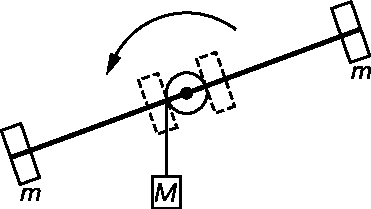
\includegraphics[width=0.9\linewidth]{fyz_fig401.pdf}
      \caption{\uv{Setrvačnost vůči rotaci} závisí na délce příslušných ramen
              (\cite[s.~10000]{Feynman01})}
      \label{fyz:fig401}
    \end{figure}  

    To je analogie zákona o tom, že hybnost je hmotnost krát rychlost. Místo rychlosti je tu úhlová
    rychlost a vidíme, že místo hmotnosti tu vystupuje něco nového, co nazýváme \textbf{momentem
    setrvačnosti} \(I\) - je to analogie hmotnosti. Rovnice (\ref{fyz:eq669}) a (\ref{fyz:eq670})
    vyjadřují, že rotující těleso má setrvačné vlastnosti, které závisí nejen na hmotnostech částic,
    ale i na jejich vzdálenostech od osy. Takže máme-li dvě tělesa stejné hmotnosti a posuneme-lij e
    dál od osy, jejich rotační setrvačnost se zvětší. Lze to snadno ukázat na zařízení, jež je
    znázorněno na obr. \ref{fyz:fig401}, kde rychlému pádu závaží \(M\) brání dlouhé vahadlo, jímž
    se musí otáčet. Nejdříve jsou závaží \(m\) umístěna blízko osy a \(M\) padá s určitým
    zrychlením. Když však změníme moment setrvačnosti tím, že závaží m posuneme dále od osy, vidíme,
    že \(M\) má mnohem menší zrychlení než předtím, neboť těleso má mnohem větší setrvačnost vůči
    rotaci. Moment setrvačnosti je projevem této setrvačnosti proti otáčení. Je roven součtu
    příspěvků všech hmotností vynásobených druhou mocninou jejich vzdáleností od osy otáčení.

    Mezi hmotností a momentem setrvačnosti je jeden „dramatický“ rozdíl. Hmotnost tělesa se nemění,
    ale jeho moment setrvačnosti se může změnit. Kdybychom se postavili na podstavec otáčející se
    bez tření a v roztažených rukách bychom drželi závaží, přičemž bychom se pomalu otáčeli, mohli
    bychom přitažením rukou změnit moment setrvačnosti, aniž by se naše hmotnost změnila. Jakmile to
    uděláme, začnou se dít v důsledku zákona o zachování momentu hybnosti podivuhodné věci. Je-li
    vnější moment sil roven nule, zůstává moment hybnosti (moment setrvačnosti krát omega)
    konstantní. Nejdříve jsme se otáčeli s velkým momentem setrvačnosti \(I_1\) a malou úhlovou
    rychlostí \(ω_1\), a moment hybnosti byl \(I_1ω_1\). Pak jsme přitažením rukou změnili moment
    setrvačnosti, řekněme na menší hodnotu \(I_2\). Součin \(Iω\), jenž musí zůstat nezměněn (neboť
    moment hybnosti musí zůstat stejný), je pak roven \(I_2ω_2\). Takže \(I_1ω_1=I_2ω_2\). Z toho
    vyplývá, že když se zmenší moment setrvačnosti, musí se zvětšit úhlová rychlost.


  \section{Příklady a cvičení}\label{fyz:IchapXVIIIsecVI}
%---------------------------------------------------------------------------------------------------